\documentclass[]{book}
\usepackage{lmodern}
\usepackage{amssymb,amsmath}
\usepackage{ifxetex,ifluatex}
\usepackage{fixltx2e} % provides \textsubscript
\ifnum 0\ifxetex 1\fi\ifluatex 1\fi=0 % if pdftex
  \usepackage[T1]{fontenc}
  \usepackage[utf8]{inputenc}
\else % if luatex or xelatex
  \ifxetex
    \usepackage{mathspec}
  \else
    \usepackage{fontspec}
  \fi
  \defaultfontfeatures{Ligatures=TeX,Scale=MatchLowercase}
\fi
% use upquote if available, for straight quotes in verbatim environments
\IfFileExists{upquote.sty}{\usepackage{upquote}}{}
% use microtype if available
\IfFileExists{microtype.sty}{%
\usepackage[]{microtype}
\UseMicrotypeSet[protrusion]{basicmath} % disable protrusion for tt fonts
}{}
\PassOptionsToPackage{hyphens}{url} % url is loaded by hyperref
\usepackage[unicode=true]{hyperref}
\hypersetup{
            pdftitle={Space-use and Demography of Pronghorn in Utah},
            pdfauthor={Veronica A. Winter},
            pdfborder={0 0 0},
            breaklinks=true}
\urlstyle{same}  % don't use monospace font for urls
\usepackage{natbib}
\bibliographystyle{ecology}
\usepackage{color}
\usepackage{fancyvrb}
\newcommand{\VerbBar}{|}
\newcommand{\VERB}{\Verb[commandchars=\\\{\}]}
\DefineVerbatimEnvironment{Highlighting}{Verbatim}{commandchars=\\\{\}}
% Add ',fontsize=\small' for more characters per line
\usepackage{framed}
\definecolor{shadecolor}{RGB}{248,248,248}
\newenvironment{Shaded}{\begin{snugshade}}{\end{snugshade}}
\newcommand{\KeywordTok}[1]{\textcolor[rgb]{0.13,0.29,0.53}{\textbf{#1}}}
\newcommand{\DataTypeTok}[1]{\textcolor[rgb]{0.13,0.29,0.53}{#1}}
\newcommand{\DecValTok}[1]{\textcolor[rgb]{0.00,0.00,0.81}{#1}}
\newcommand{\BaseNTok}[1]{\textcolor[rgb]{0.00,0.00,0.81}{#1}}
\newcommand{\FloatTok}[1]{\textcolor[rgb]{0.00,0.00,0.81}{#1}}
\newcommand{\ConstantTok}[1]{\textcolor[rgb]{0.00,0.00,0.00}{#1}}
\newcommand{\CharTok}[1]{\textcolor[rgb]{0.31,0.60,0.02}{#1}}
\newcommand{\SpecialCharTok}[1]{\textcolor[rgb]{0.00,0.00,0.00}{#1}}
\newcommand{\StringTok}[1]{\textcolor[rgb]{0.31,0.60,0.02}{#1}}
\newcommand{\VerbatimStringTok}[1]{\textcolor[rgb]{0.31,0.60,0.02}{#1}}
\newcommand{\SpecialStringTok}[1]{\textcolor[rgb]{0.31,0.60,0.02}{#1}}
\newcommand{\ImportTok}[1]{#1}
\newcommand{\CommentTok}[1]{\textcolor[rgb]{0.56,0.35,0.01}{\textit{#1}}}
\newcommand{\DocumentationTok}[1]{\textcolor[rgb]{0.56,0.35,0.01}{\textbf{\textit{#1}}}}
\newcommand{\AnnotationTok}[1]{\textcolor[rgb]{0.56,0.35,0.01}{\textbf{\textit{#1}}}}
\newcommand{\CommentVarTok}[1]{\textcolor[rgb]{0.56,0.35,0.01}{\textbf{\textit{#1}}}}
\newcommand{\OtherTok}[1]{\textcolor[rgb]{0.56,0.35,0.01}{#1}}
\newcommand{\FunctionTok}[1]{\textcolor[rgb]{0.00,0.00,0.00}{#1}}
\newcommand{\VariableTok}[1]{\textcolor[rgb]{0.00,0.00,0.00}{#1}}
\newcommand{\ControlFlowTok}[1]{\textcolor[rgb]{0.13,0.29,0.53}{\textbf{#1}}}
\newcommand{\OperatorTok}[1]{\textcolor[rgb]{0.81,0.36,0.00}{\textbf{#1}}}
\newcommand{\BuiltInTok}[1]{#1}
\newcommand{\ExtensionTok}[1]{#1}
\newcommand{\PreprocessorTok}[1]{\textcolor[rgb]{0.56,0.35,0.01}{\textit{#1}}}
\newcommand{\AttributeTok}[1]{\textcolor[rgb]{0.77,0.63,0.00}{#1}}
\newcommand{\RegionMarkerTok}[1]{#1}
\newcommand{\InformationTok}[1]{\textcolor[rgb]{0.56,0.35,0.01}{\textbf{\textit{#1}}}}
\newcommand{\WarningTok}[1]{\textcolor[rgb]{0.56,0.35,0.01}{\textbf{\textit{#1}}}}
\newcommand{\AlertTok}[1]{\textcolor[rgb]{0.94,0.16,0.16}{#1}}
\newcommand{\ErrorTok}[1]{\textcolor[rgb]{0.64,0.00,0.00}{\textbf{#1}}}
\newcommand{\NormalTok}[1]{#1}
\usepackage{longtable,booktabs}
% Fix footnotes in tables (requires footnote package)
\IfFileExists{footnote.sty}{\usepackage{footnote}\makesavenoteenv{long table}}{}
\usepackage{graphicx,grffile}
\makeatletter
\def\maxwidth{\ifdim\Gin@nat@width>\linewidth\linewidth\else\Gin@nat@width\fi}
\def\maxheight{\ifdim\Gin@nat@height>\textheight\textheight\else\Gin@nat@height\fi}
\makeatother
% Scale images if necessary, so that they will not overflow the page
% margins by default, and it is still possible to overwrite the defaults
% using explicit options in \includegraphics[width, height, ...]{}
\setkeys{Gin}{width=\maxwidth,height=\maxheight,keepaspectratio}
\IfFileExists{parskip.sty}{%
\usepackage{parskip}
}{% else
\setlength{\parindent}{0pt}
\setlength{\parskip}{6pt plus 2pt minus 1pt}
}
\setlength{\emergencystretch}{3em}  % prevent overfull lines
\providecommand{\tightlist}{%
  \setlength{\itemsep}{0pt}\setlength{\parskip}{0pt}}
\setcounter{secnumdepth}{5}
% Redefines (sub)paragraphs to behave more like sections
\ifx\paragraph\undefined\else
\let\oldparagraph\paragraph
\renewcommand{\paragraph}[1]{\oldparagraph{#1}\mbox{}}
\fi
\ifx\subparagraph\undefined\else
\let\oldsubparagraph\subparagraph
\renewcommand{\subparagraph}[1]{\oldsubparagraph{#1}\mbox{}}
\fi

% set default figure placement to htbp
\makeatletter
\def\fps@figure{htbp}
\makeatother

\usepackage{booktabs}

\title{Space-use and Demography of Pronghorn in Utah}
\author{Veronica A. Winter}
\date{2021-03-12}

\begin{document}
\maketitle

{
\setcounter{tocdepth}{1}
\tableofcontents
}
\textbf{What is space-use?}

The distribution and abundance of individual animals across a
heterogeneous landscape is expected to influence population dynamics as
a whole (Morales et al. 2010). An animal's movement through a landscape
reflects its perception and reaction to its environment. This movement
of individuals occurs in response to the shifting distribution of
resources across space and time and ultimately translates into patterns
of survival and reproductive success (Gaillard et al. 2010). Space-use
behavior reflects spatial and temporal trade-offs an animal must
navigate to meet fitness requirements, such as balancing nutritional
uptake against predator avoidance (Rosenzweig 1991), and the spatial
distribution of individuals is directly linked to dynamics of the
population (Fig. 1; Kernohan et al. 2001). The resulting space-use
patterns of an individual can offer insights into behavioral and
demographic processes affecting population viability, but despite the
apparent connection, the link between demographic rates and movement
ecology is rarely empirically examined in the literature.

\textbf{Why is this important?}

Animals exhibit distinct classes of movement behaviors that can vary at
different spatiotemporal scales. Migration is one class of annual
movement behavior in which individuals will travel between home ranges
at seasonal intervals (Dingle and Drake 2007). This alternation between
seasonal ranges is hypothesized to be driven by benefits such as reduced
predation risk, mating, and increasing access to higher-quality forage
(Avgar et al. 2014). Range residency and nomadism are additional classes
of movement patterns driven by phenology and landscape factors which
dictate range occupancy and alter population distribution strategies
(Mueller and Fagan 2008, Mueller et al. 2011). It is by examining these
movement patterns that we may gain a deeper understanding of the
contribution of an individual's behavior to population distributions and
viability at the seasonal and annual spatiotemporal scale.

\textbf{Why pronghorn?}

The pronghorn, \textbf{Antilocapra americana}, is North Americas'
\emph{only} extant endemic ungulate, and has historical ranges within
prairie, shrubland-steppe, and desert habitat in the continental west
(Berger 2004). Recent population declines across this species wide
geographic range have sparked a growing interest in investigating their
previously understudied ecology (Beale and Smith 1970, Byers 1997, Poor
et al. 2012). Pronghorn population dynamics are being altered by
anthropogenic disturbance and climate change (Gedir et al. 2015). These
changes are often accompanied by arrested landscape-scale movements.

\textbf{The project}

I will be investigating pronghorn ecology across space and time while
linking variability in space-use patterns to demographic consequences.
To do this, I will be using GPS data colelcted over the past several
years. By identifying the links between space-use and demography, we
will be able to recognize key influential factors that can inform future
management of pronghorn as well as other migratory species that share
the landscape.

\chapter{Establishing a SQL data base}\label{Ch}

\textbf{Pronghorn background}

The pronghorn, \emph{Antilocapra americana}, is North Americas' only
extant endemic ungulate, and has historical ranges within prarie,
shrubland -steppe, and desert habitat in the contnental west. Recent
population declines across this species geographic range have sparked a
growing interest in investigating their previously understudied ecology.
In Utah, it is currently unknown if this ungulate still undergoes an
annual migration or its seasonal range distribution.

Starting in 2016, the UDWR had begun fitting pronghorn with GPS collars
as a part of their migration initiative. Using this data, I am to
quantify space-use beahvior of pronghorn in Utah by delineating between
migratory, resident, and nomiadic behavior of individuals in order to
gain a better understanding of their population-level distribution
patterns.

Here, I will be constructing a SQLIte database containing their
individual information (sex, mortality, age, etc.) and tracking
information (gps coordinates, sattilites, etc.) using the \texttt{DBI}
and \texttt{RSQLite} packages.

\textbf{Getting started} First, install and load packages as follows:

\begin{Shaded}
\begin{Highlighting}[]
\CommentTok{#install.packages("RSQLite")}
\CommentTok{#install.packages("DBI")}

\CommentTok{# Load in package}
\KeywordTok{library}\NormalTok{(DBI)}
\CommentTok{# }\AlertTok{NOTE}\CommentTok{: as per Hadley Wickham, we often don't need all the tols in 'RSQLite', so we will laod in 'DBI' and call 'RSQLite' as needed.}
\end{Highlighting}
\end{Shaded}

\textbf{Database structure}

Getting data from collarborators is no small task. For now, the databse
structure will appear as follows and updates will be made as data is
secured:

\begin{figure}

{\centering 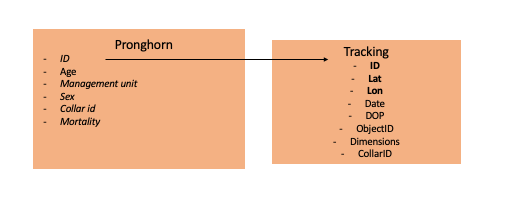
\includegraphics[width=0.5\linewidth]{/Users/vermanica/Documents/VW_Final_Prj_RS/Final_prj_RS/Database_arrangement} 

}

\caption{Pronghorn data base structure}\label{fig:logo}
\end{figure}

First: establish the data base connection and load in appropriate .csv's

\begin{Shaded}
\begin{Highlighting}[]
\NormalTok{### Est. database connection ---}
\NormalTok{pronghorn <-}\StringTok{ }\KeywordTok{dbConnect}\NormalTok{(}\DataTypeTok{drv =}\NormalTok{ RSQLite}\OperatorTok{::}\KeywordTok{SQLite}\NormalTok{(), }\CommentTok{# Location of saved db}
  \StringTok{"/Users/vermanica/Documents/VW_Final_Prj_RS/Final_prj_RS/Data/pronghorn.db"}\NormalTok{)}

\KeywordTok{class}\NormalTok{(pronghorn)}
\end{Highlighting}
\end{Shaded}

\begin{verbatim}
## [1] "SQLiteConnection"
## attr(,"package")
## [1] "RSQLite"
\end{verbatim}

Now, let's set up the two tables.

\begin{Shaded}
\begin{Highlighting}[]
\NormalTok{## Import data to the db ---}

\CommentTok{# Table 1 .csv}
\NormalTok{ph <-}\StringTok{ }\KeywordTok{read.csv}\NormalTok{(}\StringTok{"/Users/vermanica/Documents/VW_Final_Prj_RS/Final_prj_RS/Data/PH_data/processed_data/ph.csv"}\NormalTok{)}

\CommentTok{# Table 2 .csv}
\NormalTok{track <-}\StringTok{ }\KeywordTok{read.csv}\NormalTok{(}\StringTok{"/Users/vermanica/Documents/VW_Final_Prj_RS/Final_prj_RS/Data/PH_data/processed_data/tracking.csv"}\NormalTok{)}
\end{Highlighting}
\end{Shaded}

```

Table 1: \textbf{Pronghorn} This is a table that contains all the fixed
attributes of the collared individuals.

Table 1: \textbf{Tracking} - This is a table that contains all the GPS
attributes of the collared individuals.

With this data, I hope to be able to delineate migration, determine
seasonal home ranges, and eventually perform a survival analysis and
model demographics for the Utah population..

Last, let's do some checks to make sure everything worked

\begin{Shaded}
\begin{Highlighting}[]
\CommentTok{#Check that it worked ---}
\KeywordTok{dbGetQuery}\NormalTok{(}\DataTypeTok{conn =}\NormalTok{ pronghorn, }\DataTypeTok{statement =} \StringTok{"SELECT* FROM pronghorn LIMIT 10;"}\NormalTok{)}
\end{Highlighting}
\end{Shaded}

\begin{verbatim}
##           ID CollarID mortality sex age_class             unit
## 1  PR20F0054    45948         0   F     adult      North Slope
## 2  PR17F0009    40440         0   F     adult          Plateau
## 3  PR18F0002    42330         0   F     adult Southwest Desert
## 4  PR20M0004    46037         0   M     adult      West Desert
## 5  PR20F0016    46042         0   F     adult      West Desert
## 6  PR17M0022    40504         0   M     adult          Plateau
## 7  PR20M0002    46021         0   M      <NA>      West Desert
## 8  PR17F0018    40456         0   F     adult          Plateau
## 9  PR20F0014    46029         0   F      <NA>      West Desert
## 10 PR17U0004    40495         0   U     adult          Plateau
\end{verbatim}

\begin{Shaded}
\begin{Highlighting}[]
\KeywordTok{dbGetQuery}\NormalTok{(}\DataTypeTok{conn =}\NormalTok{ pronghorn, }\DataTypeTok{statement =} \StringTok{"SELECT* FROM tracking LIMIT 5;"}\NormalTok{)}
\end{Highlighting}
\end{Shaded}

\begin{verbatim}
##          ID      lat       lon dop ObjectID NumSats Dimension           dt
## 1 PR20F0054 40.98637 -109.2109 1.0 22032734       8         3 6/17/20 4:00
## 2 PR17F0009 38.32036 -111.7530 0.8 22027496       9         3 6/17/20 4:00
## 3 PR18F0002 38.10193 -112.9547 1.0 22029823       7         3 6/17/20 4:00
## 4 PR20M0004 40.85842 -112.8552 1.0 22030458       8         3 6/17/20 4:00
## 5 PR20F0016 40.75581 -112.9860 0.8 22032586       9         3 6/17/20 4:00
\end{verbatim}

Looks good! We are all set.

\chapter{Literature}\label{literature}

Here is a review of existing methods.

\chapter{Methods}\label{methods}

We describe our methods in this chapter.

\chapter{Applications}\label{applications}

Some \emph{significant} applications are demonstrated in this chapter.

\section{Example one}\label{example-one}

\section{Example two}\label{example-two}

\chapter{Final Words}\label{final-words}

We have finished a nice book.

\bibliography{book.bib,packages.bib}

\end{document}
